% Issue #81, part "Hybrid architecture and rationale"; owner: vks-g. Input from
% reports/phase2/main.tex (tikz with arrows.meta and positioning is loaded there).
% Numbers: results/metrics/fd001_hybrid_study.csv, fd001_hybrid_value_test.json and
% fd001_hybrid_gate_by_stage.csv (notebooks/phase2/09_hybrid.ipynb, #68).
% Table: tables/hybrid_value_cv.tex, generated by scripts/prepare_results_tables.py.
% Settings: configs/hybrid_gated.yaml, configs/hybrid_two_stage.yaml; code: src/rul/models/hybrid.py.

\section{Hybrid Architectures}
\label{sec:hybrid}

The Phase~1 features and the sequence encoders see an engine's history in
different ways. The engineered features summarize at most the last 20 cycles
with fixed statistics: a rolling mean, a slope and a health index over 5, 10
and 20 cycles. A sequence encoder reads 30 cycles in order and learns its own
summary. The two views overlap, but they are not the same, and a hybrid can add
value only if each carries something the other misses. Fusing handcrafted
features with an LSTM has helped before: Chen et al.~\cite{Chen2021machine}
lowered the FD001 RMSE of their LSTM from 15.43 to 14.81 by adding features,
and Jin et al.~\cite{Jin2022bilstm} fused a feature stream with a
bidirectional LSTM. We build two hybrids that ask different questions
(Fig.~\ref{fig:hybrids}). Hybrid~A asks whether one network can learn when to
trust each view. Hybrid~B asks whether a learned sequence representation adds
anything to the strongest machine-learning model, gradient-boosted trees on
the engineered features. It is also the literal combination of a machine
learning and a deep learning model.

\begin{figure}[t]
\centering
\resizebox{\columnwidth}{!}{%
\begin{tikzpicture}[
  box/.style={draw, rounded corners=2pt, align=center, font=\footnotesize,
              minimum height=7mm, inner sep=3pt},
  dat/.style={box, fill=black!6},
  lab/.style={font=\scriptsize, midway, above},
  ttl/.style={font=\footnotesize\bfseries, anchor=west},
  >={Stealth[length=2mm]}]
% Hybrid A
\node[ttl] at (-0.8,1.3) {A: gated fusion (one network, trained end to end)};
\node[dat] (wa) at (0,0.55) {window\\$[B,30,15]$};
\node[dat] (fa) at (0,-0.75) {features\\$[B,151]$};
\node[box] (lstm) at (2.3,0.55) {LSTM\\$1{\times}64$};
\node[box] (mlp) at (2.3,-0.75) {MLP\\width 32};
\node[box] (gate) at (5.4,-0.1) {gate $g$\\$z=g\,h_s+(1{-}g)\,h_f$};
\node[box] (ha) at (7.75,-0.1) {linear\\head};
\node[box] (ya) at (9.0,-0.1) {RUL};
\draw[->] (wa) -- (lstm);
\draw[->] (fa) -- (mlp);
\draw[->] (lstm.east) -- node[lab, above, sloped]{$h_s$} (gate.west);
\draw[->] (mlp.east) -- node[lab, below, sloped]{$h_f$} (gate.west);
\draw[->] (gate) -- (ha);
\draw[->] (ha) -- (ya);
% Hybrid B
\node[ttl] at (-0.8,-1.85) {B: two-stage (stage 1 deep, stage 2 boosted trees)};
\node[dat] (wb) at (0,-2.6) {window\\$[B,30,15]$};
\node[dat] (fb) at (0,-3.9) {features\\$[B,151]$};
\node[box] (enc) at (2.3,-2.6) {LSTM $1{\times}64$\\cross-fitted};
\node[box] (cat) at (5.4,-3.25) {$[\,$features; embedding$\,]$\\$[B,215]$};
\node[box] (xgb) at (7.75,-3.25) {XGBoost};
\node[box] (yb) at (9.0,-3.25) {RUL};
\draw[->] (wb) -- (enc);
\draw[->] (enc.east) -- node[lab, above right, pos=0.35]{64} (cat.west);
\draw[->] (fb.east) -- (cat.west);
\draw[->] (cat) -- (xgb);
\draw[->] (xgb) -- (yb);
\end{tikzpicture}}
\caption{The two hybrids on FD001. Both use the tuned LSTM of
Section~\ref{sec:architecture} as the sequence branch and the 151 engineered
features at the window's last cycle (cycle index, 15 scaled sensors, and
rolling mean, slope and health index over 5, 10 and 20 cycles). In B, each
training engine's embedding comes from an LSTM that never saw that engine.}
\label{fig:hybrids}
\end{figure}

\subsection{Hybrid A: Gated Fusion}
Hybrid~A embeds the window with the LSTM and the engineered features with a
small MLP, both to 64 dimensions, and mixes the two embeddings with a learned
gate per dimension (Section~\ref{sec:theory}). Gating comes from multimodal
fusion~\cite{Arevalo2017gated}. Unlike concatenation, it can weight the
branches differently for each window, for example the features early in life
and the sequence near failure. The network trains end to end with the shared
trainer, windows, cap and early stopping of Section~\ref{sec:architecture}.
The only new setting is the width of the feature branch. Among 32, 64 and 128,
we kept the smallest within one fold standard deviation of the best, which
is 32. Switching the gate for concatenation or for one branch alone gives the
ablation variants of Section~\ref{sec:ablations}.

\subsection{Hybrid B: Two-Stage}
Hybrid~B trains the LSTM on RUL first, then feeds its 64-dimensional window
embedding to XGBoost~\cite{Chen2016xgboost} together with the 151 engineered
features. The difficulty is leakage between the stages. An LSTM embeds its own
training engines better than it will embed new ones. If XGBoost trained on
those embeddings, it would learn to trust them more than they deserve. We
therefore \emph{cross-fit} the embeddings, as stacking does with out-of-fold
predictions~\cite{Wolpert1992stacked}. The training engines are split into
three groups by engine, and each group is embedded by an LSTM trained on the
other two. A fourth LSTM, trained on every training engine, embeds new
engines at prediction time. All four use the tuned LSTM's settings. XGBoost
uses depth 3, 200 trees, learning rate 0.1, row and column subsampling of 0.8
and a minimum child weight of 5. These settings were tuned on the features
alone, which, if anything, favours the branch over the hybrid and makes the
value test harder to pass.

\subsection{The Value Test}
The criteria were fixed in the project tracker before any hybrid was
trained. A hybrid adds value over its best single branch only if at least one
of the following holds: (1)~the paired bootstrap 95\% interval on the RMSE
difference over engines lies below zero~\cite{Efron1993introduction};
(2)~a Holm-corrected~\cite{Holm1979simple} Wilcoxon signed-rank
test~\cite{Wilcoxon1945individual} on the per-engine errors gives $p<0.05$,
with the hybrid's median error lower; or (3)~its RMSE varies less across
seeds, with a mean that is no worse. Otherwise the result is null. The best
single branch is the one with the lowest cross-validated error. For Hybrid~A,
and for plain concatenation as a reference, it is the better of the LSTM and
the feature MLP. For Hybrid~B, it is the best of XGBoost on the features,
XGBoost on the embeddings alone and the LSTM. In cross-validation, a held-out
engine's error is its RMSE over cycles with true RUL $\leq130$. Every model
runs at seeds 42, 43 and 44, and the three comparisons form one Holm family.
Section~\ref{sec:validation} repeats the same test on the official test set.

\subsection{Cross-Validated Results}

\begin{table*}[t]
\centering
\caption{Value test of the hybrids in cross-validation (FD001, 3 folds, seeds
42--44). Hybrid and Branch: root mean square over the 100 held-out engines of
each engine's RMSE on cycles with true RUL $\leq130$, mean $\pm$ s.d.\ over
seeds. $\Delta$: hybrid minus branch, paired bootstrap 95\% CI.
$p_\mathrm{Holm}$: Wilcoxon signed-rank on per-engine error, Holm-corrected
over the three comparisons. (1)--(3): the value-test criteria.}
\label{tab:hybrid_value_cv}
\footnotesize
% Generated by scripts/prepare_results_tables.py from
% results/metrics/fd001_hybrid_value_test.json (#68). Do not edit by hand.
\begin{tabular}{@{}llcccccccl@{}}
\hline
Hybrid & Best branch & Hybrid & Branch & $\Delta$ [95\% CI] & $p_\mathrm{Holm}$ & (1) & (2) & (3) & Verdict \\
\hline
Hybrid A, gated & LSTM & 16.61 $\pm$ 0.24 & 16.90 $\pm$ 0.98 & $-$0.29 [$-$2.19, $+$1.49] & 0.054 & no & no & yes & passes (3) \\
Concatenation & LSTM & 16.92 $\pm$ 0.11 & 16.90 $\pm$ 0.98 & $+$0.02 [$-$1.91, $+$1.84] & 0.13 & no & no & no & null \\
Hybrid B, two-stage & XGBoost, features & 14.67 $\pm$ 0.29 & 14.68 $\pm$ 0.18 & $-$0.01 [$-$0.58, $+$0.55] & 0.46 & no & no & no & null \\
\hline
\end{tabular}

\end{table*}

\begin{figure}[t]
\centering
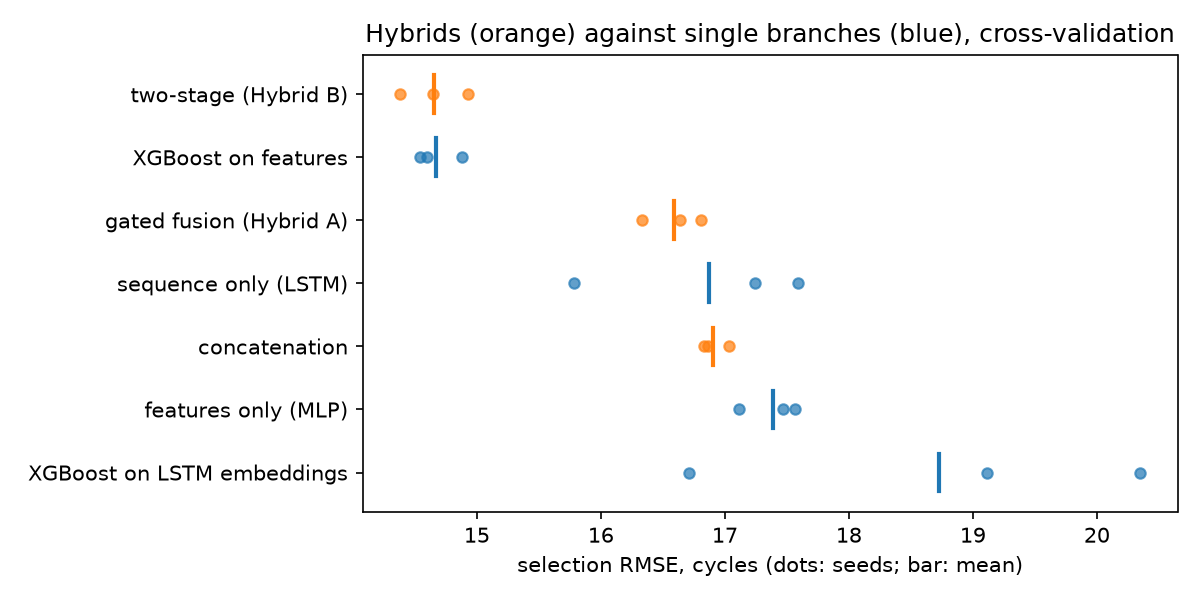
\includegraphics[width=\columnwidth]{../../results/figures/fd001_hybrid_comparison.png}
\caption{Hybrids (orange) against single branches (blue) in cross-validation:
selection RMSE at each of the three seeds (dots) and its mean (bar).}
\label{fig:hybrid_comparison}
\end{figure}

Fig.~\ref{fig:hybrid_comparison} ranks the seven models by mean selection
RMSE over the three seeds. The two-stage hybrid (14.65) and XGBoost on the
features (14.67) lead, followed by gated fusion (16.59), the LSTM (16.87),
concatenation (16.91), the feature MLP (17.39) and XGBoost on the LSTM
embeddings alone (18.73). On FD001, boosted trees on engineered features are
the strongest model, and every network is about two cycles or more behind
them. Table~\ref{tab:hybrid_value_cv} applies the value test.

\emph{Hybrid~B gives a null result.} Its difference from XGBoost on the
features is $-0.01$ cycles, with an interval of $-0.58$ to $+0.55$, and it is
better on 43 of the 100 engines. The LSTM embeddings add nothing measurable to
what the features already carry. On their own they are the weakest input, and
the most seed-dependent (16.71 to 20.35 across seeds).

\emph{Hybrid~A passes, on criterion~(3) only.} Its RMSE varies much less
across seeds than the LSTM's (s.d.\ 0.24 against 0.98), with a lower mean
(16.61 against 16.90). The other two criteria fail: the interval includes
zero, and the corrected $p$ is 0.054 (0.018 before correction). This pass
needs a caveat. The LSTM was tuned at seed 42, where it scores 15.79, against
17.62 and 17.29 at seeds 43 and 44, and that inflates its spread. On the two
untuned seeds alone, the gated hybrid still leads (16.50 against 17.46) and is
better on 63 of 100 engines. Plain concatenation also beats the LSTM there
(16.94), so most of the gain comes from adding the features at all, and the
gate adds a little on top. The gain is not uniform over life. Adding the
features helps near failure (late-stage RMSE 9.62 against 11.09) and in mid
life (20.06 against 21.69), but costs accuracy early in life (19.39 against
15.88).

\emph{The gate gives no stable story.} Averaged over its 64 entries, the
gate stays between 0.48 and 0.56 at every life stage and seed, and its trend
with RUL changes direction from seed to seed. On average, neither branch dominates at
any stage. As Section~\ref{sec:theory} warns, a gate value is a mixing weight
and not a contribution, so the branch ablations, not the gate, are the
evidence for what each input adds.

In short, cross-validation gives a small but stable gain for gated fusion over
the LSTM, and none for the two-stage model over boosted trees. Both hybrids
were then frozen with the settings above and scored once on the official
test set (Section~\ref{sec:validation}).
